\documentclass[12pt]{article}
\usepackage[frenchb]{babel} 
\usepackage[T1]{fontenc}
\usepackage[utf8]{inputenc}
%\usepackage{lmodern} 
\usepackage{graphicx}
\usepackage{caption}
\usepackage{multirow}
\usepackage[top=2.5cm, bottom=2.5cm, left=2.5cm , right=2.5cm]{geometry}
%\usepackage{amsmath}
%\usepackage{amsthm}
%\usepackage{amsfonts}
\usepackage{empheq}
\usepackage{setspace}
\usepackage{hyperref}
\hypersetup{pdftitle = {ELE8812 - Rapport de laboratoire}, pdfauthor={Julien Antoine}}
\usepackage{color}
\usepackage{subfigure}
\usepackage{fancyvrb}
\usepackage{SIunits}
\usepackage{numprint}
\usepackage{enumitem}
\usepackage{calc}
\usepackage{listings}
\usepackage{float}
\usepackage{cellspace}
\cellspacetoplimit=4pt
\cellspacebottomlimit=4pt

% ----------------------------------- FANCY HEADER -----------------------------------
\usepackage{fancyhdr}
\pagestyle{fancy}
\renewcommand{\headrulewidth}{0.5pt}
%\fancyhead[C]{\textbf{page \thepage}} 
\fancyhead[L]{}
\fancyhead[R]{Rapport de laboratoire 3}

\renewcommand{\footrulewidth}{0.5pt}
\fancyfoot[C]{\textbf{\thepage}} 
\fancyfoot[L]{Polytechnique Montréal}
\fancyfoot[R]{ELE8812}
% ------------------------------------------------------------------------------------


\providecommand{\e}[1]{\ensuremath{\cdot 10^{#1}}}
\newcommand{\question}{\noindent$\bullet$\;\;}
\newcommand{\eau}{\ensuremath{\text{H}_2 \text{O}}}
\newcommand{\dio}{\ensuremath{\text{CO}_2}}
%\addto\captionsfrancais{\renewcommand{\chaptername}{Labo}}

\definecolor{mygreen}{RGB}{28,172,0} % color values Red, Green, Blue
\definecolor{mylilas}{RGB}{170,55,241}

\begin{document}

\lstset{language=Matlab,%
	%basicstyle=\color{red},
	breaklines=true,%
	morekeywords={matlab2tikz},
	keywordstyle=\color{blue},%
	morekeywords=[2]{1}, keywordstyle=[2]{\color{black}},
	identifierstyle=\color{black},%
	stringstyle=\color{mylilas},
	commentstyle=\color{mygreen},%
	showstringspaces=false,%without this there will be a symbol in the places where there is a space
	numbers=left,%
	numberstyle={\tiny \color{black}},% size of the numbers
	numbersep=9pt, % this defines how far the numbers are from the text
	emph=[1]{for,end,break},emphstyle=[1]\color{red}, %some words to emphasise
	%emph=[2]{word1,word2}, emphstyle=[2]{style},    
}

\hyphenation{HyperLogLog experimental techno-logy according develop-ment}

\begin{titlepage}
\newcommand{\HRule}{\rule{\linewidth}{0.5mm}} % Defines a new command for the horizontal lines, change thickness here

%-------------------------------------------------------------------------------------
%	LOGO SECTION
%-------------------------------------------------------------------------------------
\centering

\includegraphics[width = 0.33\textwidth]{../../logo}\\[5cm] 
\centering
%-------------------------------------------------------------------------------------
%	TITLE SECTION
%-------------------------------------------------------------------------------------
\HRule \\[0.4cm]
{ \huge \bfseries ELE8812 -- Rapport de laboratoire 4}\\[0.4cm] 
{ \Large \bfseries Analyse multirésolution}\\
\HRule \\[1cm]
%-------------------------------------------------------------------------------------
%	AUTHOR SECTION
%-------------------------------------------------------------------------------------
\begin{minipage}{0.45\textwidth}
\begin{center} 
\large
Julien \textsc{Antoine}\\
1813026
\end{center}
\end{minipage}
~
\begin{minipage}{0.45\textwidth}
\begin{center} 
\large
Maxime \textsc{Schmitt}\\
1719088
\end{center}
\end{minipage}\\[8cm]
%-------------------------------------------------------------------------------------
%	DATE SECTION
%-------------------------------------------------------------------------------------
\begin{center}
{\Large 23 mars 2016}
\end{center}
%-------------------------------------------------------------------------------------
\vfill 
\end{titlepage}

%\tableofcontents


\section{Introduction}
L'objectif de ce laboratoire est de se familiariser avec la transformée en ondelettes
rapide et certaines de ses applications. On s'intéresse dans la première partie à son
utilisation pour la compression d'images puis dans la seconde partie à son utilité pour
la correction de défauts localisés. Tout au long de ce laboratoire, on utilisera
différents types d'ondelettes afin de se sensibiliser sur l'effet de ce choix sur le
résultat de la transformée.

\section{Transformée en ondelettes rapide d'une image}
\subsection{Transformée directe et transformée inverse}

On s'intéresse dans un premier temps à l'ondelette de Haar, les réponses impulsionnelles
des filtres de codage-décodage en sous-bandes relatifs à celle-ci sont données dans la
figure~\ref{impulsedb1}. On retrouve ensuite la Transformée en Ondelettes Rapide (TOR)
de l'image \textit{Lenna.tif} utilisant 3 niveaux d'échelle dans la figure~\ref{TORdb1}.
On reconstruit ensuite l'image en effectuant la TOR inverse, le résultat est affiché en
vis-à-vis avec l'image originale dans la figure~\ref{reconstructiondb1}. On constate
qu'on ne distingue pas à l'oeil nu de différences entre l'image originale et celle
reconstruite. De plus, une vérification numérique sur la différence entre ces deux
images (maximum de la valeur absolue de la différence pixel par pixel) révèle qu'elles
sont bien identiques.

Ces mêmes opérations, effectuées cette fois avec l'ondelette, db4 sont présentées sur
les figures~\ref{impulsedb4},~\ref{TORdb4} et~\ref{reconstructiondb4}.

On remarque des différences entre les TOR utilisant l'ondelette de Haar
(figure~\ref{TORdb1}) et celles utilisant l'ondelette db4 (figure~\ref{TORdb4}). Cette
dernière semble conserver dans les coefficients de détail des détails de plus petite
taille que ceux conservés dans le cas de l'ondelette de Haar. Cela est logique puisque
le choix d'une fonction donnée pour l'ondelette correspond à un choix d'échelle
correspondant : l'ondelette de Haar (db1) correspond à des détails "plus gros" que ceux
de l'ondelette db4.

\begin{figure}[H]
	\centering
	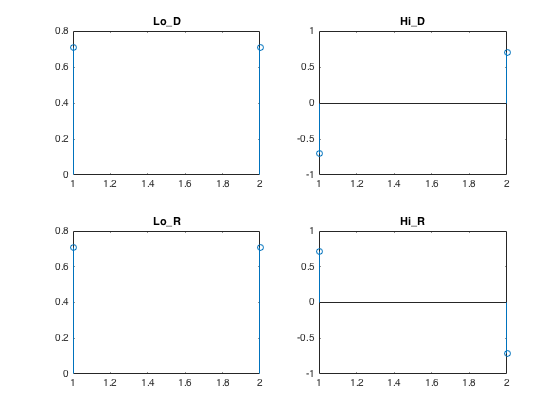
\includegraphics[width = \textwidth]{images/3-1-reponsesImpulsionnelles-db1}
	\captionsetup{justification=centering}
	\caption{Réponses impulsionnelles des filtres de codage-décodage en sous-bandes de l'ondelette de \textbf{Haar}}
	\label{impulsedb1}
\end{figure}

\begin{figure}[H]
	\centering
	\centerline{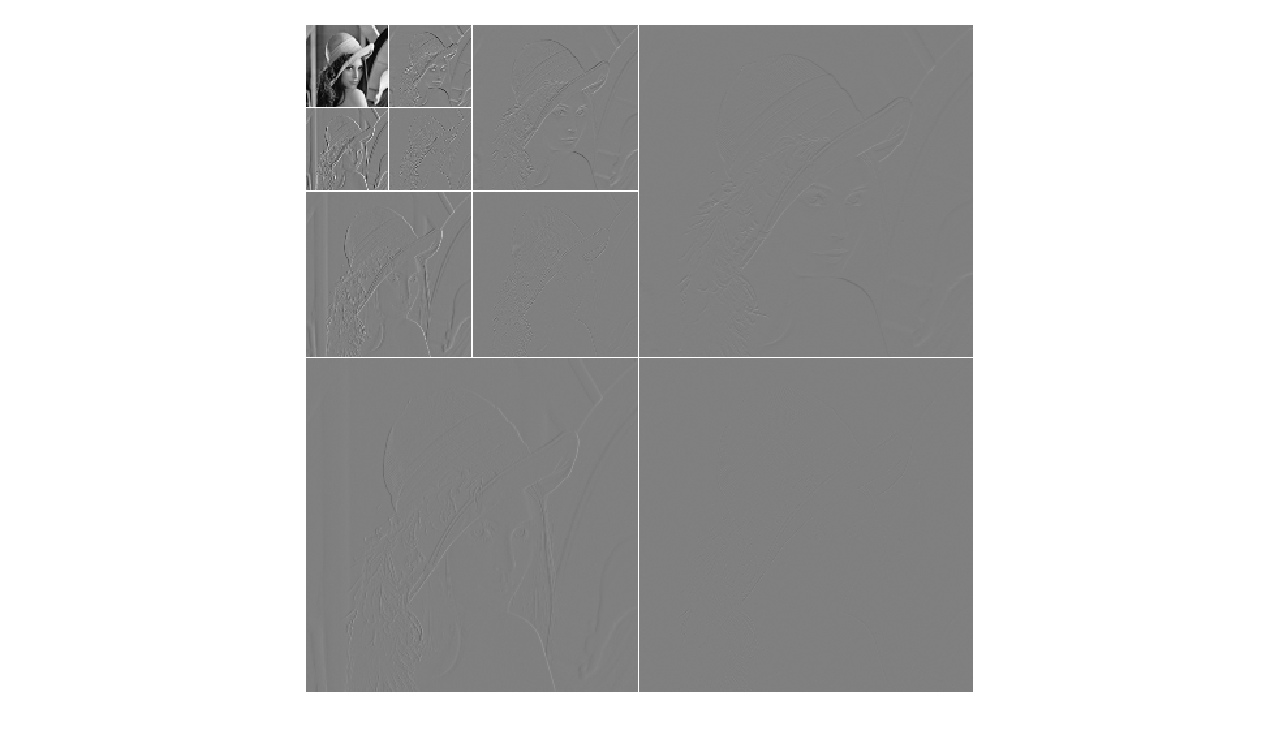
\includegraphics[width = 1.6\textwidth]{images/3-1-db1}}
	\captionsetup{justification=centering}
	\caption{Transformée en Ondelettes Rapide à 3 niveaux d'échelle de l'image \textit{Lenna.tif} avec l'ondelette de \textbf{Haar}}
	\label{TORdb1}
\end{figure}

\begin{figure}[H]
	\centering
	\hspace*{-2.15cm}
	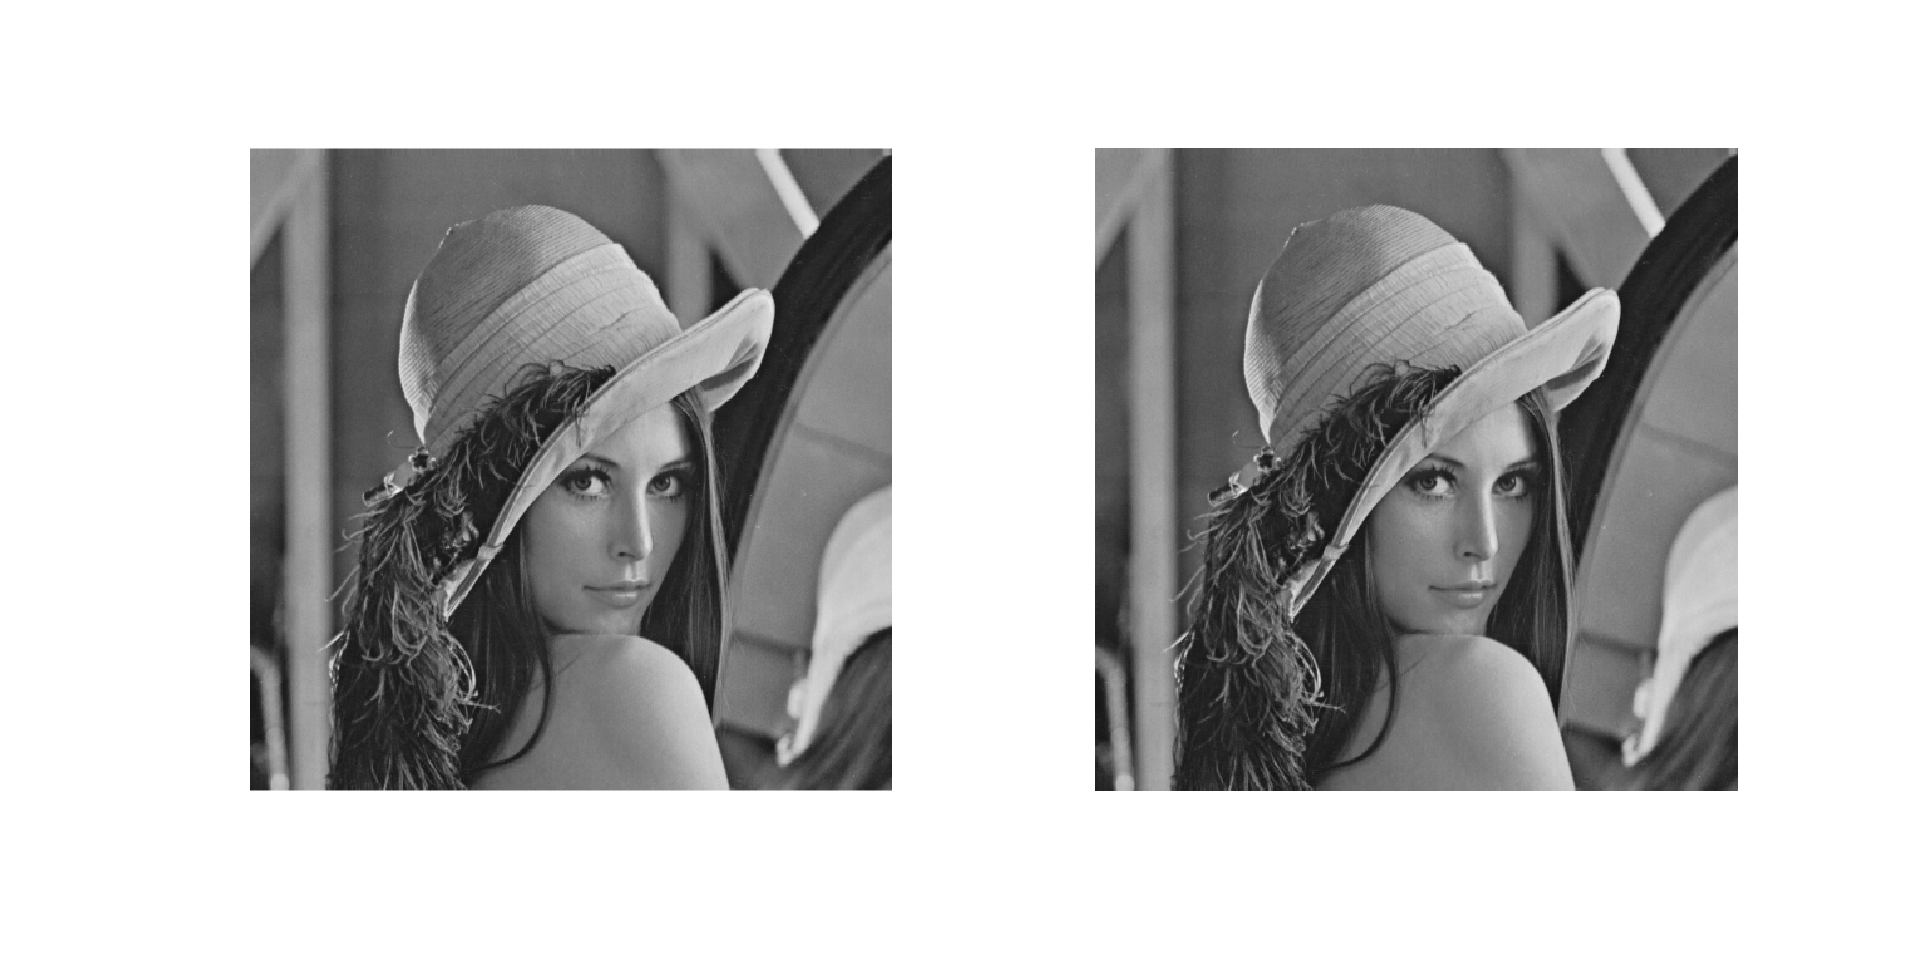
\includegraphics[width = 1.2\textwidth]{images/3-1-reconstruction-db1}	\captionsetup{justification=centering}
	\caption{Comparaison de l'image originale (à gauche) et de l'image reconstruite avec l'ondelette de \textbf{Haar} (à droite)}
	\label{reconstructiondb1}
\end{figure}

\begin{figure}[H]
	\centering
	\centerline{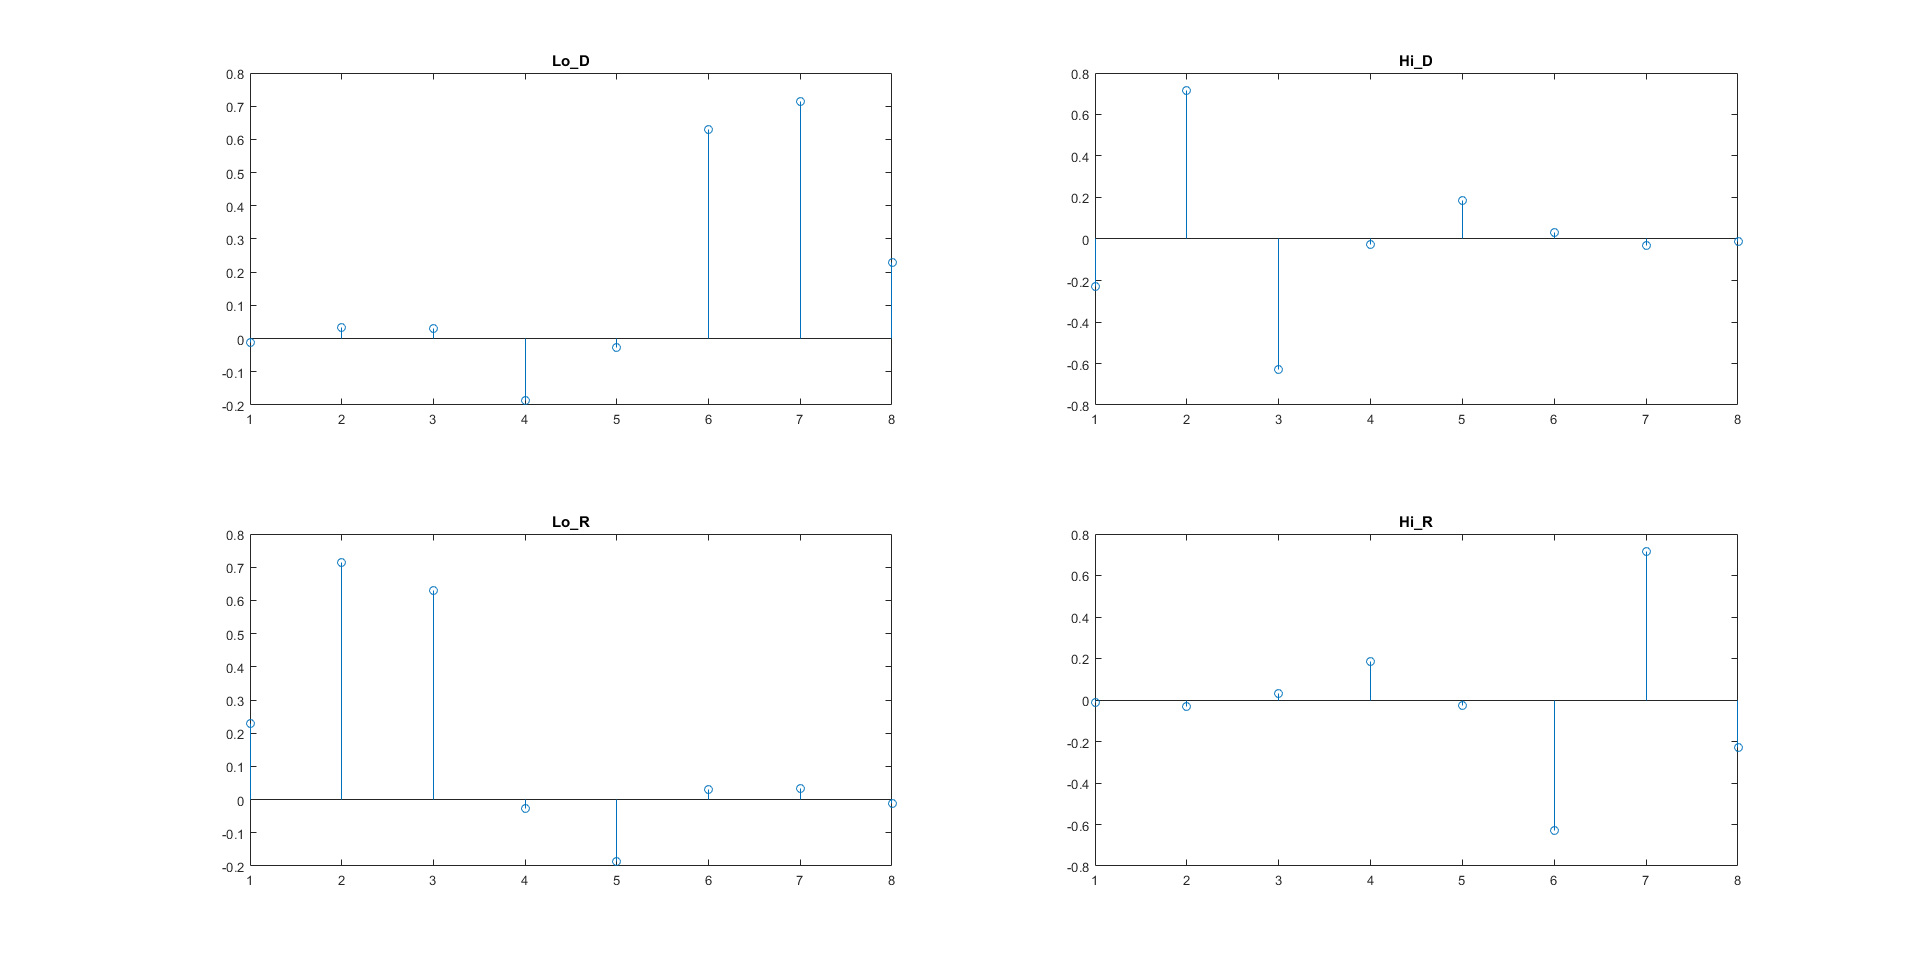
\includegraphics[width = 1.3\textwidth]{images/3-1-reponsesImpulsionnelles-db4}}
	\captionsetup{justification=centering}
	\caption{Réponses impulsionnelles des filtres de codage-décodage en sous-bandes de l'ondelette de \textbf{Haar}}
	\label{impulsedb4}
\end{figure}

\begin{figure}[H]
	\centering
	\centerline{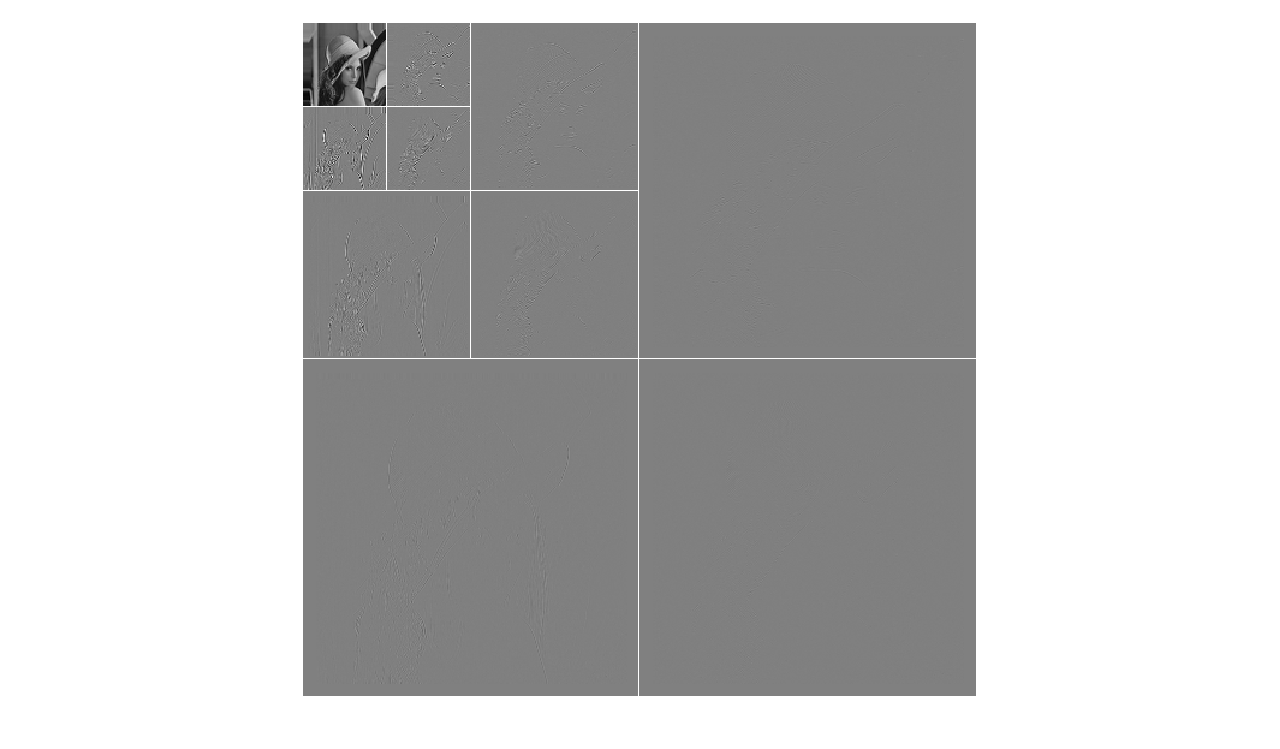
\includegraphics[width = 1.6\textwidth]{images/3-1-db4}}
	\captionsetup{justification=centering}
	\caption{Transformée en Ondelettes Rapide à 3 niveaux d'échelle de l'image \textit{Lenna.tif} avec l'ondelette \textbf{db4}}
	\label{TORdb4}
\end{figure}

\begin{figure}[H]
	\centering
	\hspace*{-2.15cm}
	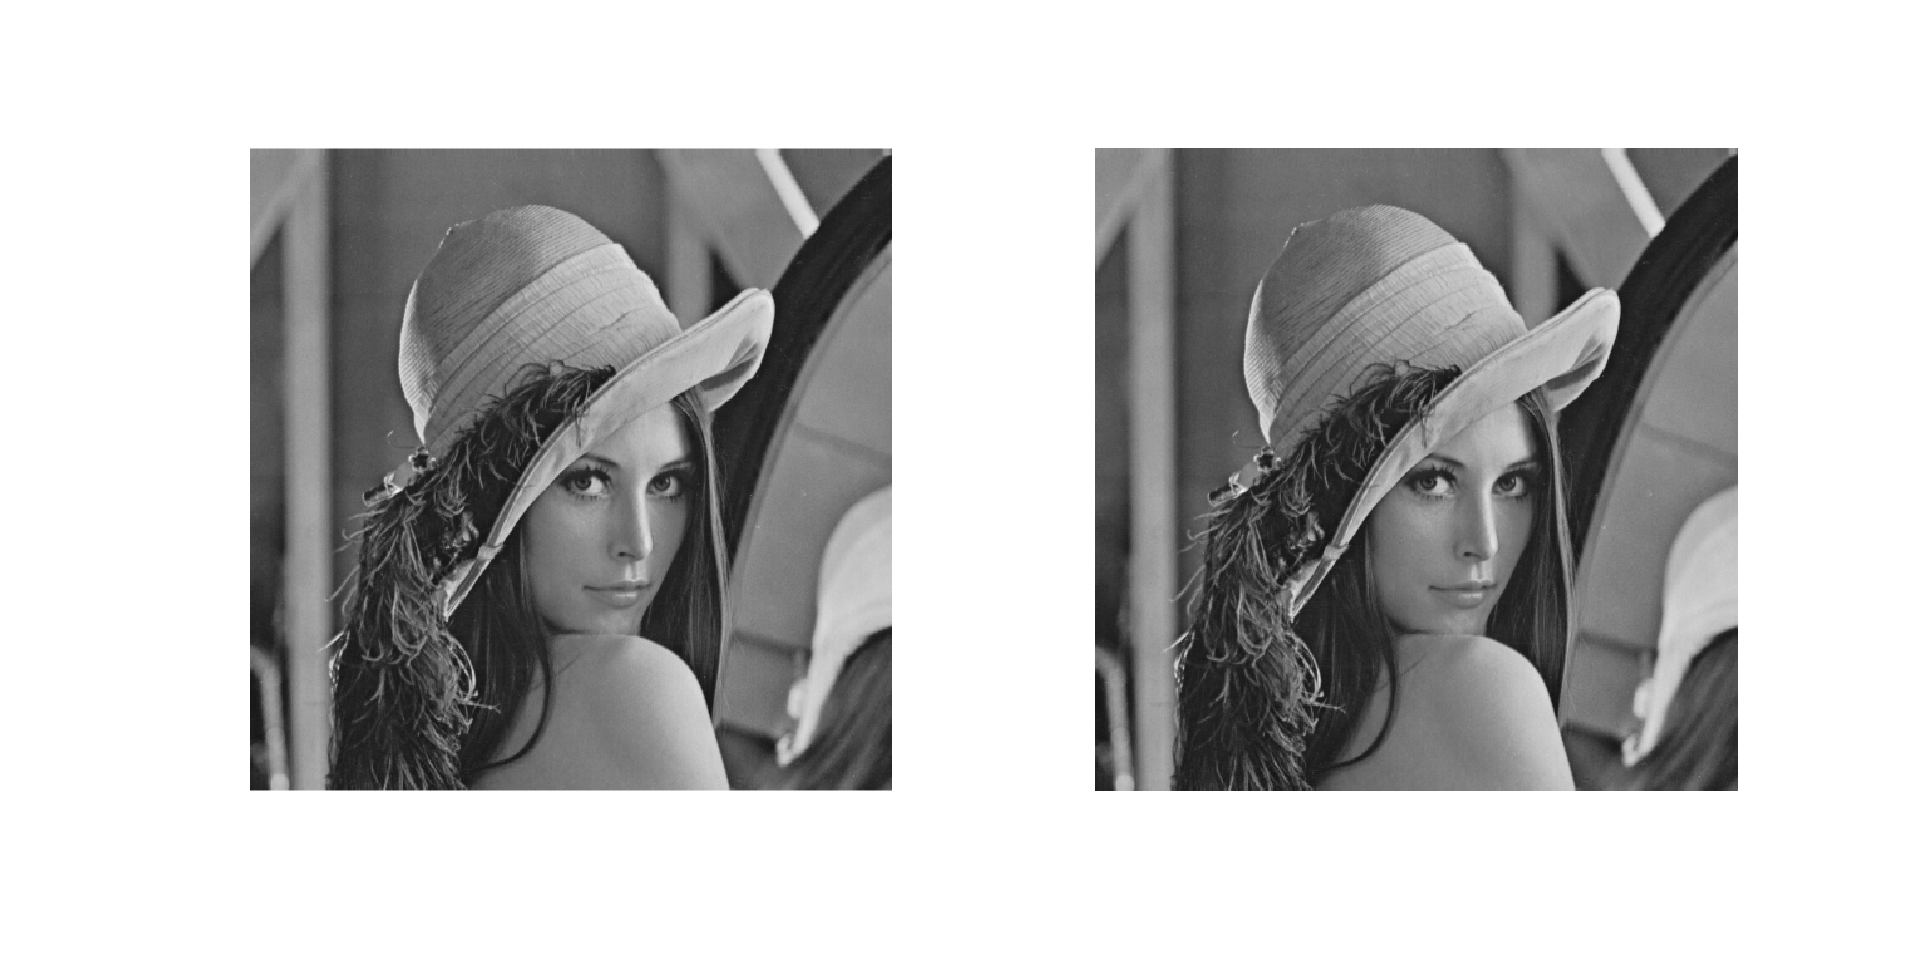
\includegraphics[width = 1.2\textwidth]{images/3-1-reconstruction-db4}	\captionsetup{justification=centering}
	\caption{Comparaison de l'image originale (à gauche) et de l'image reconstruite avec l'ondelette de \textbf{db4} (à droite)}
	\label{reconstructiondb4}
\end{figure}

\subsection{Utilisation pour la compression}

On effectue la compression de l'image de la façon décrite dans l'énoncé et on observe
alors qu'on peut obtenir un taux de compression très important en ne dégradant que peu
l'image en choisissant un bon seuil mais également que si on choisit un seuil trop grand
on obtient alors un taux de compression sensiblement meilleur mais la qualité de l'image
s'en retrouve dégradée de façon plus importante également. Les
figures~\ref{compression10} et~\ref{compression200} illustrent ce propos puisqu'on a sur
la première une image bien compressée (taux de compression de 85.45\%) mais avec une
erreur introduite par la compression faible (erreur quadratique moyenne de 2.69\%) alors
que sur la seconde on a une image davantage compressée (taux de compression de 98.36\%)
mais l'erreur introduite est elle aussi bien plus importante (erreur quadratique
moyenne de 11.91\%) et les artefacts liés à la compression sont alors visibles à l'oeil
nu. Les artefacts visibles sont liés au fait que l'on a perdu des informations liées
aux hautes fréquences dans l'image.

\begin{figure}[H]
	\centering
	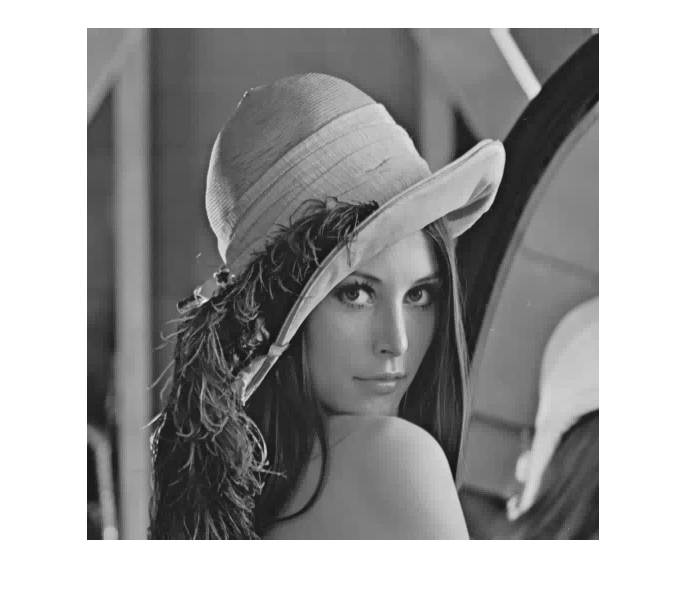
\includegraphics[width = \textwidth]{images/3-2-seuil10}	\captionsetup{justification=centering}
	\caption{Image compressée avec une valeur de seuil de 10 (compression de 85.45\% et erreur de 2.69\%)}
	\label{compression10}
\end{figure}

\begin{figure}[H]
	\centering
	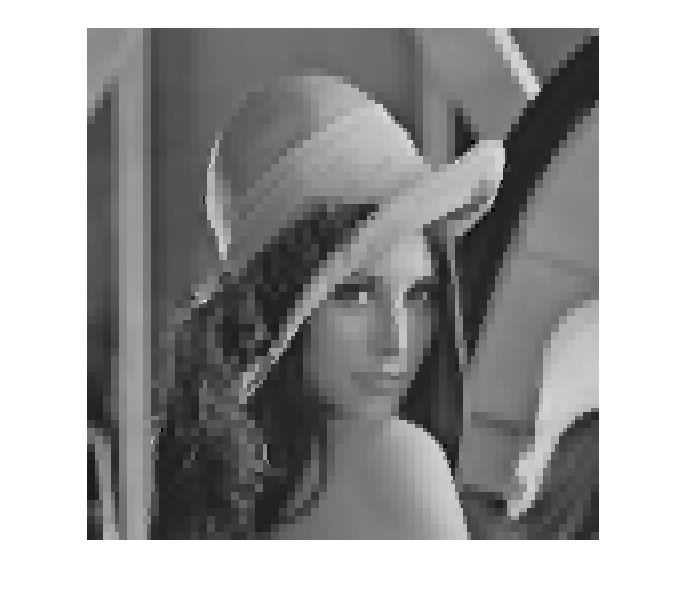
\includegraphics[width = \textwidth]{images/3-2-seuil200}	\captionsetup{justification=centering}
	\caption{Image compressée avec une valeur de seuil de 200 (compression de 98.36\% et erreur de 11.91\%)}
	\label{compression200}
\end{figure}

\section{Correction de défauts localisés}
\subsection{Traitement des coefficients de la décomposition}
En calculant la TOR de l'image \textsf{Lena\_r.tif}, on remarque que la ligne blanche, étant verticale, apparaît uniquement dans les coefficients verticaux (\autoref{fig:4Tor}).

\begin{figure}[!h]
	\centering
	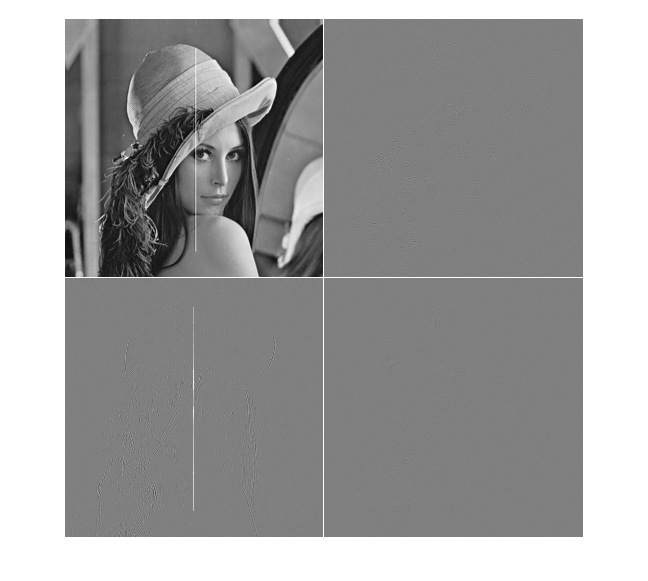
\includegraphics[width = 0.7\textwidth]{images/4TOR}
	\caption{Transformée en ondelettes rapide}
	\label{fig:4Tor}
\end{figure}

Pour enlever cette ligne blanche, on met à zéro les coefficients verticaux
correspondant à la position de la ligne. La \autoref{fig:4-1} représente le meilleur
résultat, obtenu avec les paramètres $n=4$ et $\delta=1$, où $n$ est le nombre
d'échelles, et $\delta$ le nombre de pixels autour de la ligne.

\begin{figure}[!h]
	\centering
	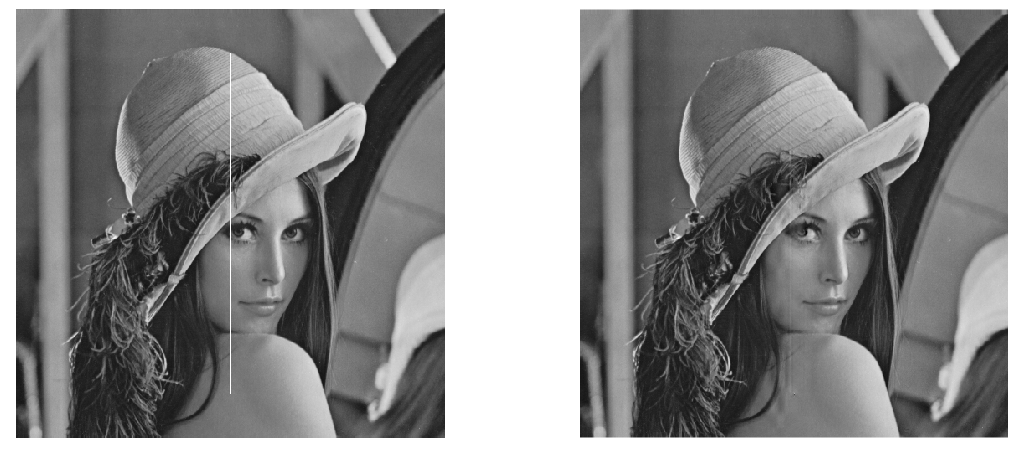
\includegraphics[width = 0.7\textwidth]{images/4-1db4copie}
	\caption{Ondelette \texttt{db4}, $n=4$ et $\delta=1$}
	\label{fig:4-1}
\end{figure}


\subsection{Effet du type d'ondelette}
Intéressons-nous maintenant à l'influence du type d'ondelette utilisé. La figure \autoref{fig:42haar} montre que le résultat obtenu avec l'ondelette de Haar est moins bon qu'avec l'ondelette \texttt{db4}. L'ondelette \texttt{sym6} (figure \ref{fig:42sym6}) fait mieux que Haar, et donne un résultat un peu similaire à \texttt{db4}.

\begin{figure}[!h] 
	\centering
	\subfigure[Ondelette de Haar, $n=3$ et $\delta=1$]{
		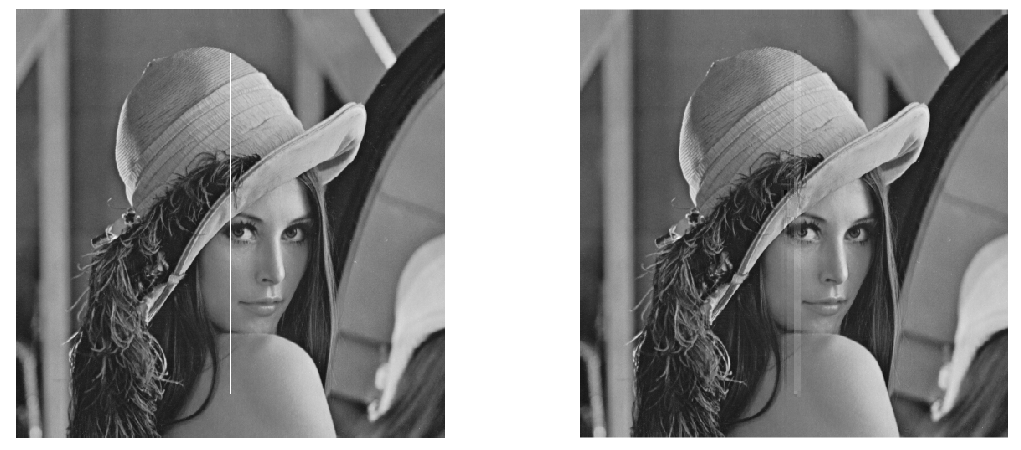
\includegraphics[width = 0.7\textwidth]{images/4-2haarcopie}
		\label{fig:42haar} }
	\quad
	\subfigure[Ondelette \texttt{sym6}, $n=4$ et $\delta=1$]{
		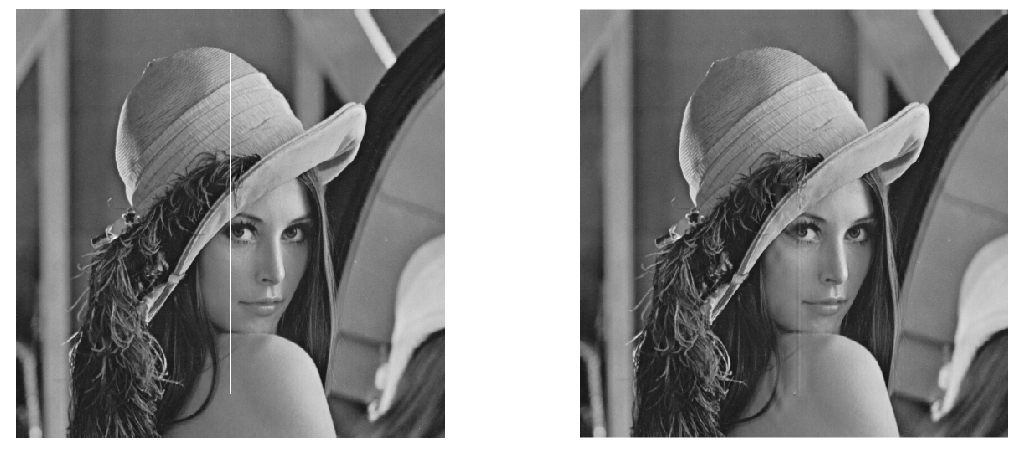
\includegraphics[width = 0.7\textwidth]{images/4-2sym6copie}
		\label{fig:42sym6} }
	\caption{Influence du type d'ondelette utilisé} 
	\label{}
\end{figure}



\subsection{Effet de l'orientation du défaut}
Etudions à présent l'effet de l'orientation du défaut. L'image considérée comporte une ligne non plus verticale, mais oblique. Dès lors, on ne peut plus se limiter à éliminer les coefficients verticaux uniquement, il faut considérer tous les types de coefficients. Cependant, après quelques expérimentations, il est apparu qu'en ne considérant pas les coefficients horizontaux, le résultat obtenu était meilleur. Il est plus compliqué d'obtenir un résultat aussi satisfaisant que lorsque le trait était vertical, comme le montre la \autoref{fig:43}.

\begin{figure}[!h]
	\centering
	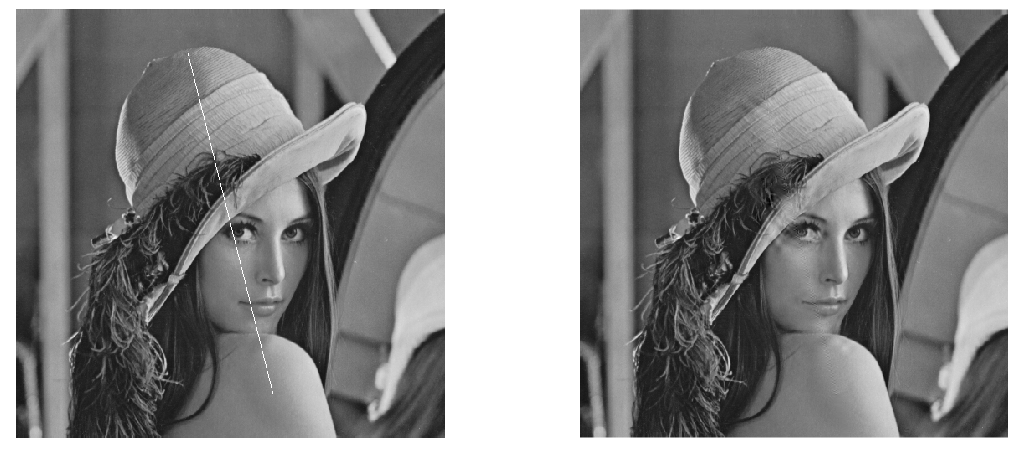
\includegraphics[width = 0.7\textwidth]{images/43sym6copie2}
	\caption{Ondelette \texttt{sym6}, $n=4$ et $\delta=2$}
	\label{fig:43}
\end{figure}


\subsection{Effet du type d'image}
Changeons d'image, et appliquons la même transformation que précédemment. On constate à
l'aide de la TOR que les coefficients horizontaux ne sont pas très importants au niveau
du trait blanc, alors que pour l'herbe et le mur blanc derrière ils le sont. Il est
donc préférable de ne jouer que sur les coefficients verticaux et diagonaux, et ainsi
préserver les textures de natures horizontales. La \autoref{fig:44} montre le résultat
obtenu de cette manière.

\begin{figure}[!h]
	\centering
	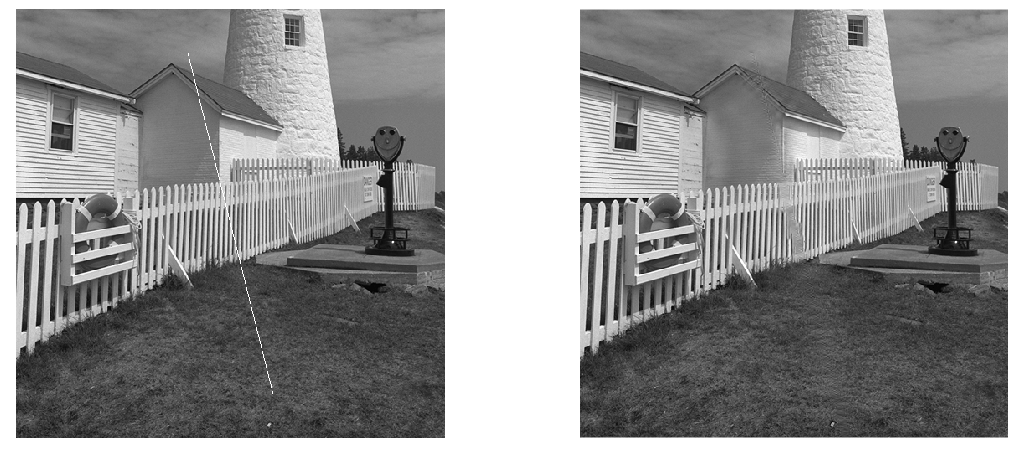
\includegraphics[width = 0.7\textwidth]{images/44sym6copie1}
	\caption{Ondelette \texttt{sym6}, $n=5$ et $\delta=2$}
	\label{fig:44}
\end{figure}

\section{Conclusion}
Dans ce laboratoire, nous avons donc pu mettre en oeuvre diverses applications de la
transformée en ondelettes et ainsi nous familiariser avec son intérêt pour des
applications en compression d'images et en correction de défauts localisés. Nous avons
pu observer son efficacité dans ces différents cas et ainsi comprendre l'important
recours à cette méthode pour l'analyse multirésolution d'images numériques.


\newpage
\section*{Annexe A - Code partie 3 : ex3.m}
\label{annexe3}
\lstinputlisting{../src/ex3.m}

\newpage
\section*{Annexe B - Code partie 4 : suppr.m}
\label{annexe4-suppr}
\lstinputlisting{../src/suppr.m}

\newpage
\section*{Annexe C - Code partie 4 : ex4.m}
\label{annexe4-12}
\lstinputlisting{../src/ex4.m}

\newpage
\section*{Annexe C - Code partie 4 : ex43.m}
\label{annexe4-3}
\lstinputlisting{../src/ex43.m}

\newpage
\section*{Annexe C - Code partie 4 : ex44.m}
\label{annexe4-3}
\lstinputlisting{../src/ex44.m}

\end{document}